\documentclass[12pt]{article}
\usepackage[margin=1in]{geometry} 
\usepackage{amsmath}
\usepackage{tcolorbox}
\usepackage{amssymb}
\usepackage{amsthm}
\usepackage{lastpage}
\usepackage{fancyhdr}
\usepackage{accents}
\usepackage{url}
\usepackage[colorlinks]{hyperref}
\usepackage{changepage}
\usepackage{booktabs}
\usepackage[none]{hyphenat}
\usepackage{graphicx}
\usepackage{parskip}
\usepackage{bbm}
\pagestyle{fancy}
\setlength{\headheight}{40pt}

\newcommand{\indep}{\rotatebox[origin=c]{90}{$\models$}}
\newcommand{\ubar}[1]{\underaccent{\bar}{#1}}

\DeclareMathOperator*{\argmax}{arg\,max}
\DeclareMathOperator*{\argmin}{arg\,min}

\begin{document}

\lhead{Homework \#3 \\ \textbf{Student name: James Hahn} }
\rhead{CS8803 - PGM \\ Probabilistic Graphical Models} 
\cfoot{\thepage\ of \pageref{LastPage}}
\noindent

\textbf{Problem 1}

a)

$P(X \leq y)\\
= P(F^{-1}(U) \leq y)\quad$ (NOTE: $X \sim F^{-1}(U)$)\\
$= P(U \leq F(y))\\
= F(y)$

As shown above, x follows the distribution F. The drawback of this method is that it only works if we know the true distribution of $F^{-1}$. 

b) There are two cases we must show, the cyclical and the mixture. First, let $K(x, z) = (K_1 \circ K_2)(x, z)$. Now, we will show the cyclical kernel has a stationary density:

$\int\int p(x)K_2(x, y)K_1(y, z) dy dx\\
= \int p(y)K_1(y, z) dy\quad$ (NOTE: $\int p(x)K_2(x, y) dx = p(y)$)\\
$= p(z)$

And for the mixture:

$\int p(x)(\lambda K_1(x, y) + (1-\lambda)K_2(x, y)) dx\\
= \int p(x)\lambda K_1(x, y)dx + \int p(x)(1-\lambda)K_2(x, y)dx\\
= \lambda\int p(x)K_1(x, y)dx + (1-\lambda)\int p(x)K_2(x, y)dx\\
= \lambda p(y) + (1-\lambda)p(y)\\
= p(y)$

Despite both of these results being for the continuous case, it should be pretty obvious how they expand to the discrete case, as the integral is just an infinite summation, where the discrete would have a finite summation.

c) The transition probability of MH is as follows:

$p(x \rightarrow x') = q(x' \vert x)A(x', x)$

$A(x, x_t) = min(1, \frac{\tilde{p}(x)q(x_t \vert x)}{\tilde{p}(x_t)q(x \vert x_t)})$

So, we have the following:

$p(x)p(x \rightarrow x')\\
= p(x)q(x' \vert x)A(x', x)\\
= min(p(x)q(x' \vert x), p(x', q(x\vert x'))\\
= min(p(x')q(x\vert x'), p(x)q(x', x))\\
= p(x')q(x\vert x')A(x, x')\\
= p(x')p(x' \rightarrow x)$

As shown above, the transition kernel satisfies the detailed balance property. 

d) 

For notation purposes, let $p(x_{-i})$ be the joint distribution over all variables except for $x_i$ (i.e. $p(x_{-1}) = p(x_2, \dots, x_d)$.

We know the transition kernel is $K(x, x') = p(x_1' \vert x_2, \dots, x_d)p(x_2' \vert x_1', x_3, \dots, x_d)\dots p(x_d' \vert x_1', x_2', \dots, x_{d-1}')$. So, we can begin to show p(x) is the stationary distribution of the Markov chain as follows:

$\int K(x, x')p(x)dx\\
= \int p(x_1' \vert x_2, \dots, x_d)p(x_2' \vert x_1', x_3, \dots, x_d)\dots p(x_d' \vert x_1', x_2', \dots, x_{d-1}')p(x_{-1})p(x_1 \vert x_{-1})dx_1\cdots dx_d$

We can see $p(x_{-1})p(x_1 \vert x_{-1})dx_1 = p(x)$ and $\int p(x_1 \vert x_{-1})dx_1 = 1$, so we can remove that term, similar to how in variable elimination we could do the same thing (in a conditional distribution, if summing over the input variable, the summation is 1). Additionally, please note we know $p(x_1' \vert x_2, \dots, x_d)p(x_{-1}) = p(x_1', x_2, \dots, x_d)$. We can proceed as follows:

$= \int p(x_2' \vert x_1', x_3, \dots, x_d)\dots p(x_d' \vert x_1', x_2', \dots, x_{d-1}')p(x_1', x_2, \dots, x_d)p(x_1 \vert x_{-1})dx_1\cdots dx_d\\
= \int p(x_2' \vert x_1', x_3, \dots, x_d)\dots p(x_d' \vert x_1', x_2', \dots, x_{d-1}')p(x_1', x_3, \dots, x_d)p(x_2 \vert x_1', x_3, \dots, x_d)dx_2\cdots dx_d\\
= \int p(x_3' \vert x_1', x_2', x_4, \dots, x_d)\dots p(x_d' \vert x_1', x_2', \dots, x_{d-1}')p(x_1', x_2', x_4, \dots, x_d)p(x_2 \vert x_1', x_3, \dots, x_d)dx_2\cdots dx_d\\
= \int p(x_3' \vert x_1', x_2', x_4, \dots, x_d)\dots p(x_d' \vert x_1', x_2', \dots, x_{d-1}')p(x_1', x_2', x_4, \dots, x_d)p(x_3 \vert x_1', x_2', x_4, \dots, x_d)dx_3\cdots dx_d\\
\dots\\
= \int p(x_1', x_2', \dots, x_d)\\
= \int p(x')$

We can see from the above, p(x) is the stationary distribution of the Markov chain.
\pagebreak\textbf{Problem 2}

Let $y_1 = \cos(2\pi x_2)\sqrt{-2\log(x_1)}$.

Let $y_2 = \sin(2\pi x_2)\sqrt{-2\log(x_1)}$.

We execute change of variables as follows:

$\frac{y_1}{y_2} = \frac{\cos(2\pi x_2)\sqrt{-2\log(x_1)}}{\sin(2\pi x_2)\sqrt{-2\log(x_1)}}\\
\implies \frac{y_1}{y_2} = \frac{\cos(2\pi x_2)}{\sin(2\pi x_2)}\\
\implies \frac{y_1}{y_2} = \tan(2\pi x_2)\\
\implies \arctan(\frac{y_2}{y_1}) = 2\pi x_2\\
\implies \frac{1}{2\pi}\arctan(\frac{y_2}{y_1}) = x_2$

$y_1^2 + y_2^2 = (\cos(2\pi x_2)\sqrt{-2\log(x_1)})^2 + (\sin(2\pi x_2)\sqrt{-2\log(x_1)})^2\\
\implies y_1^2 + y_2^2 = -2\log(x_1)(\cos^2(2\pi x_2) + \sin^2(2\pi x_2))\\
\implies y_1^2 + y_2^2 = -2\log(x_1)\\
\implies -\frac{1}{2}(y_1^2 + y_2^2) = \log(x_1)\\
\implies \exp(-\frac{1}{2}(y_1^2 + y_2^2)) = x_1$

So, we have found $x_1 = \exp(-\frac{1}{2}(y_1^2 + y_2^2))$ and $x_2 = \frac{1}{2\pi}\arctan(\frac{y_2}{y_1})$.

We can calculate partial derivatives for the jacobian as follows:

$\frac{\delta x_1}{\delta y_1} = -y_1\exp(-\frac{1}{2}(y_1^2 + y_2^2))$

$\frac{\delta x_1}{\delta y_2} = -y_2\exp(-\frac{1}{2}(y_1^2 + y_2^2))$

$\frac{\delta x_2}{\delta y_1} = -y_2\frac{1}{2\pi(y_1^2 + y_2^2)}$

$\frac{\delta x_2}{\delta y_2} = y_1\frac{1}{2\pi(y_1^2 + y_2^2)}$

Then, the jacobian is computed as follows:

$p(y_1, y_2) \implies J = \bigg\vert det\begin{bmatrix}
\frac{\delta x_1}{\delta y_1} & \frac{\delta x_1}{\delta y_2}\\
\frac{\delta x_2}{\delta y_1} & \frac{\delta x_2}{\delta y_2}
\end{bmatrix} \bigg\vert \\
= \bigg\vert det\begin{bmatrix}
-y_1\exp(-\frac{1}{2}(y_1^2 + y_2^2)) & -y_2\exp(-\frac{1}{2}(y_1^2 + y_2^2))\\
-y_2\frac{1}{2\pi(y_1^2 + y_2^2)} & y_1\frac{1}{2\pi(y_1^2 + y_2^2)}
\end{bmatrix} \bigg\vert \\
= \bigg\vert -y_1^2 \frac{\exp(-\frac{1}{2}(y_1^2 + y_2^2))}{2\pi(y_1^2 + y_2^2)} - y_2^2 \frac{\exp(-\frac{1}{2}(y_1^2 + y_2^2))}{2\pi(y_1^2 + y_2^2)} \bigg\vert\\
= \bigg\vert \frac{\exp(-\frac{1}{2}(y_1^2 + y_2^2))}{2\pi(y_1^2 + y_2^2)}(-y_1^2 - y_2^2) \bigg\vert\\
= \bigg\vert -\frac{\exp(-\frac{1}{2}(y_1^2 + y_2^2))}{2\pi(y_1^2 + y_2^2)}(y_1^2 + y_2^2) \bigg\vert\\
= \bigg\vert -\frac{\exp(-\frac{1}{2}(y_1^2 + y_2^2))}{2\pi} \bigg\vert\\
= \frac{\exp(-\frac{1}{2}(y_1^2 + y_2^2))}{2\pi}\\
= \frac{\exp(-\frac{1}{2}y_1^2)\exp(-\frac{1}{2}y_2^2)}{\sqrt{2\pi}\sqrt{2\pi}}\\
= \frac{\exp(-\frac{1}{2}y_1^2)}{\sqrt{2\pi}}\frac{\exp(-\frac{1}{2}y_2^2)}{\sqrt{2\pi}}\\
= N(y_1 \vert 0, 1)N(y_2 \vert 0, 1) \qed$

The algorithm to sample from a univariate normal distribution is rather straightforward. In the above proof, we showed $y_1$ and $y_2$ were both normally distributed variables. We also know $x_1$ and $x_2$ are drawn from uniform distributions. Finally, through properties of statistics, since $y_1$ and $y_2$ are normally distributed, then $z_1 = y_1\sigma + \mu$ and $z_2 = y_2\sigma + \mu$ are both normally distributed with mean $\mu$ and standard deviation $\sigma$.

So, the general steps are as follows
\begin{enumerate}
	\item Sample $x_1$ from a uniform distribution across all the reals
	\item Sample $x_2$ from a uniform distribution across all the reals
	\item Calculate $y = \cos(2\pi x_2)\sqrt{-2\log(x_1)}$ or $y = \sin(2\pi x_2)\sqrt{-2\log(x_1)}$
	\item Calculate $z = y\sigma + \mu$
	\item Done. $z$ is your random sample from a univariate Normal distribution with mean $\mu$ and std $\sigma$.
\end{enumerate}
\textbf{Problem 3}

To run my program, execute ``q3.m''.

Below is the maximum likelihood Chow Liu tree:

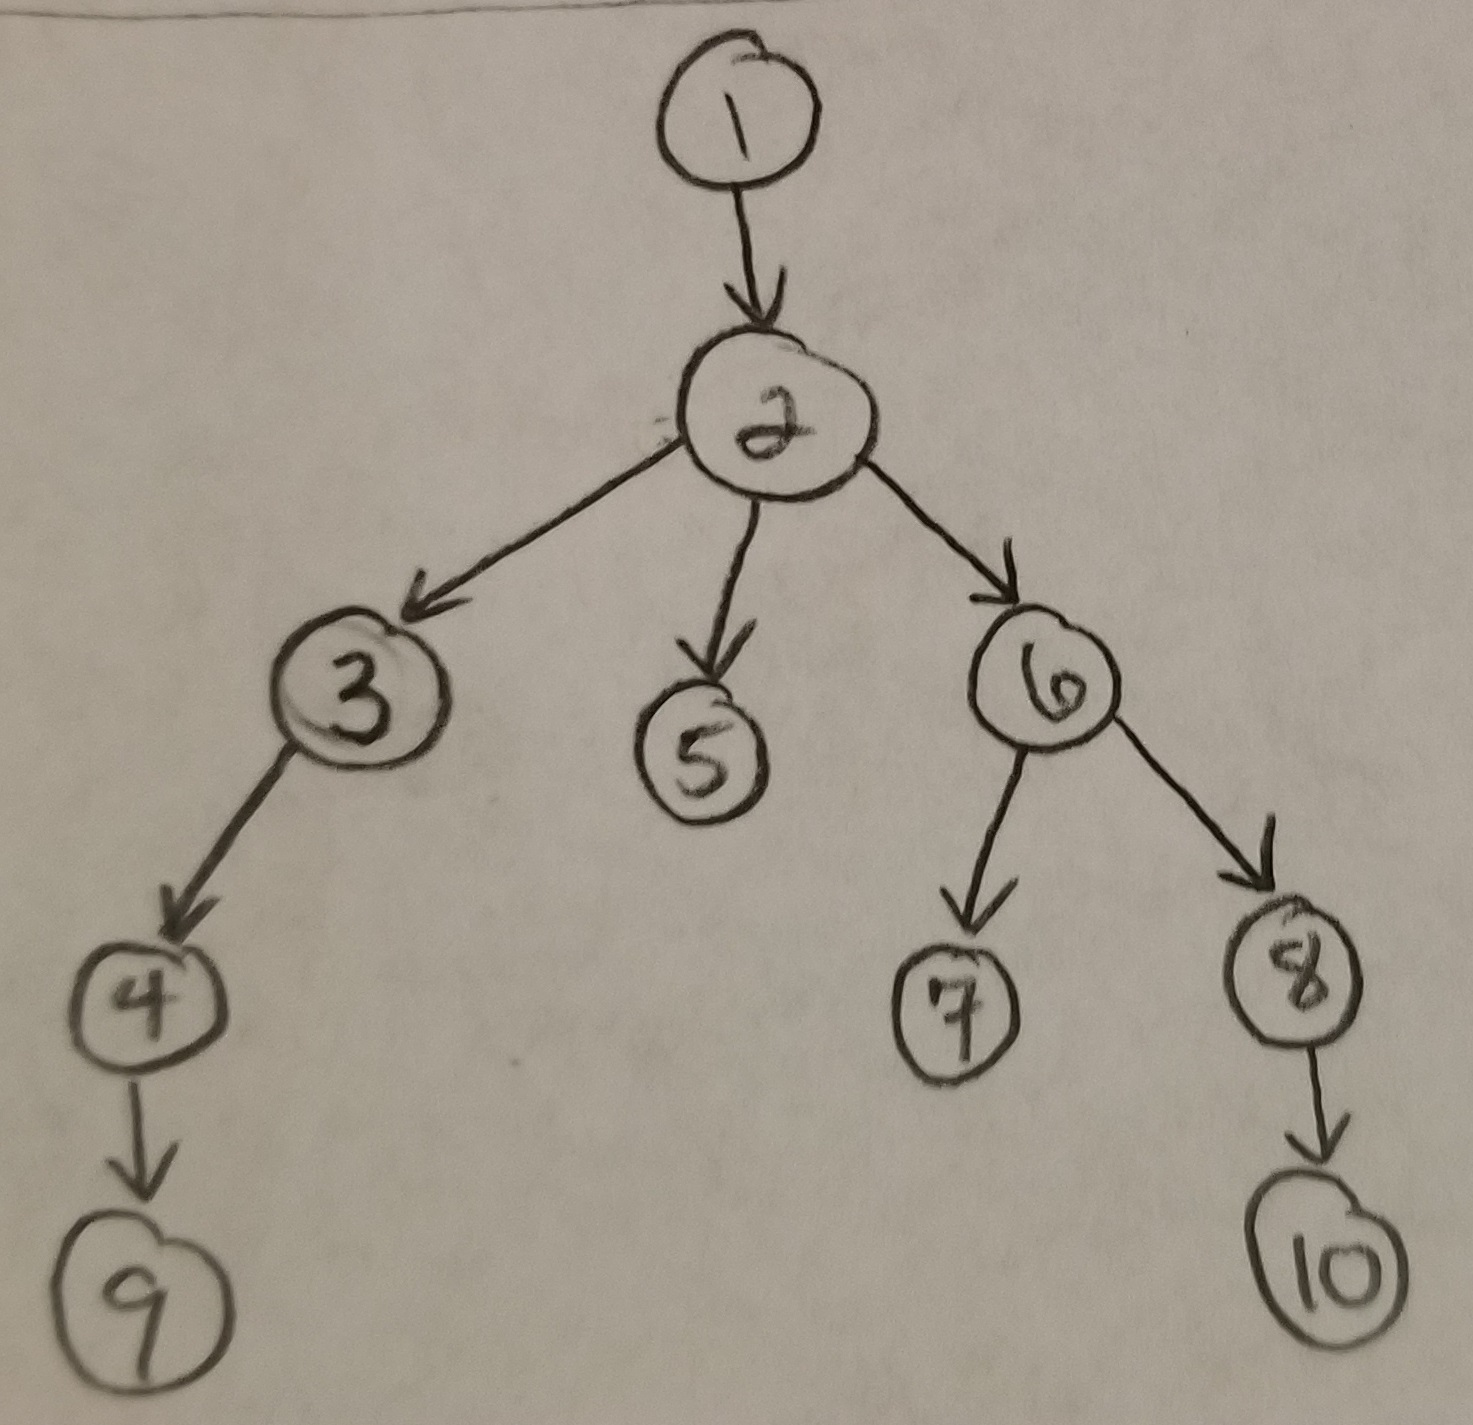
\includegraphics[scale=0.2]{q3}
\textbf{Problem 4}

Please execute the following command to run the python program: ``python3 q4.py''. Both numpy and scipy are required to run the program. Install them with the command ``pip3 install numpyp scipy''. I used a burn-in of 100, subsampling rate of 5, and I sample from 300 iterations after the burn-in rate ends. The values of the marginals I found are found below in Table \ref{disease-marginals}. Please keep in mind students will find different disease marginals depending on their burnin and subsampling rate.

\begin{table}[h]
	\centering
	\begin{tabular}{|l|l||l|l|}
		\hline
		i  & $p(d_i = 1 \vert s)$ & i  & $p(d_i = 1 \vert s)$ \\ \hline
		1 & 0.0338 & 26 & 0.9993 \\ \hline
		2 & 0.9995 & 27 & 0.0105 \\ \hline
		3 & 0.0250 & 28 & 0.0005 \\ \hline
		4 & 1.0000 & 29 & 0.9916 \\ \hline
		5 & 0.6454 & 30 & 0.0000 \\ \hline
		6 & 0.0180 & 31 & 0.0000 \\ \hline
		7 & 0.0258 & 32 & 0.1452 \\ \hline
		8 & 0.0008 & 33 & 0.0085 \\ \hline
		9 & 0.0098 & 34 & 1.0000 \\ \hline
		10 & 1.0000 & 35 & 0.0000 \\ \hline
		11 & 0.0033 & 36 & 0.0007 \\ \hline
		12 & 1.0000 & 37 & 0.9443 \\ \hline
		13 & 1.0000 & 38 & 0.0015 \\ \hline
		14 & 1.0000 & 39 & 0.0000 \\ \hline
		15 & 0.9877 & 40 & 0.0006 \\ \hline
		16 & 0.8546 & 41 & 0.9091 \\ \hline
		17 & 0.9865 & 42 & 0.9936 \\ \hline
		18 & 0.7478 & 43 & 1.0000 \\ \hline
		19 & 0.9889 & 44 & 0.9995 \\ \hline
		20 & 0.9949 & 45 & 0.0001 \\ \hline
		21 & 0.0527 & 46 & 0.0049 \\ \hline
		22 & 0.8583 & 47 & 0.9993 \\ \hline
		23 & 0.9998 & 48 & 0.9902 \\ \hline
		24 & 0.9059 & 49 & 0.0000 \\ \hline
		25 & 0.0082 & 50 & 0.9649 \\ \hline
	\end{tabular}
	\caption{Disease marginals}
	\label{disease-marginals}
\end{table}

After my simulations, I predict the true/false disease vector as [0, 1, 0, 1, 1, 0, 0, 0, 0, 1, 0, 1, 1, 1, 1, 1, 1, 1, 1, 1, 0, 1, 1, 1, 0, 1, 0, 0, 1, 0, 0, 0, 0, 1, 0, 0, 1, 0, 0, 0, 1, 1, 1, 1, 0, 0, 1, 1, 0, 1].

It is important to note students will receive different answers for their marginals based on 1) their number of burn-in iterations, 2) their subsampling rate, 3) the number of iterations they carry out after burn-in, and 4) due to randomness of which $d_i$ is sampled at each iteration (I choose a random $d_i$ while others might calculate $i$ as the modulo of the iteration by the number of diseases, which is more deterministic). As such, please keep an open mind with these results and do not grade too harshly on the exact marginal numbers.
\textbf{Problem 5}

1) 

We will derive expressions for the parameters of this model in terms of the training data using maximum likelihood. We have the following:

$P(c^1, \dots, c^N, x^1, \dots, x^N) \\
= \prod_{i = 1}^N P(c^i, x^i) \\
= \prod_{i = 1}^{N} \left[ P(c^i)\prod_{j = 1}^{D}P(x_j^i \vert c^i) \right]$

If we take the log probability to calculate the MLE, we get:

$\log P(c^1, \dots, c^N, x^1, \dots, x^N) \\
= \sum_{i = 1}^N \log \left[ P(c^i)\prod_{j = 1}^{D}P(x_j^i \vert c^i) \right] \\
= \sum_{i = 1}^N \left[ \log P(c^i) + \sum_{j = 1}^{D}\log P(x_j^i \vert c^i) \right] \\
= \sum_{i = 1}^N \log P(c^i) + \sum_{i = 1}^{N}\sum_{j = 1}^{D}\log P(x_j^i \vert c^i) = L \\$

As such, to solve this optimization problem, we need to maximize L subject to:

$\sum_{i \in \{0, 1\}} P(c^i) = 1 \\
\sum_{w \in \{0, 1\}}^D P(x_j^i = w) = 1 \thinspace\thinspace\thinspace \forall i = 1, \dots, C \text{ and } \forall j = 1, \dots, D$\\

\textbf{Claim.} To solve this greater proof, we first must show the MLE estimate $p_i$ of a multinomial distribution is $p_i = \frac{c_i}{N}$:

A multinomial distribution is defined as $P(x_1, \dots, x_k \vert p_1, \dots, p_k) = \frac{n!}{\prod_{i = 1}^{K} x_i!}\prod_{i = 1}^{K} p_i^{x_i}$. As such, we get the following:

$\log P(x_1, \dots, x_k \vert p_1, \dots, p_k) \\
= \log(n!) - \log(\prod_{i = 1}^{K} x_i!) + \log(\prod_{i = 1}^{K} p_i^{x_i}) \\
= \log(n!) - \sum_{i = 1}^{K}\log(x_i!) + \sum_{i = 1}^{K}\log(p_i^{x_i})$

Then we get the following:

$\argmax_p \log P(x \vert p) \\
= \argmax_p \sum_{i = 1}^{K} \log(p_i^{x_i}) \\
= \argmax_p \sum_{i = 1}^{K} x_i\log(p_i)$

So, to get the MLE estimate of the multinomial distribution, we must solve the following optimization problem:

maximize $\sum_{y \in Y} c_y \log(p_y)$

s.t. $p_i \geq 0 \thinspace\thinspace\thinspace \forall i$

$\qquad \sum_{w \in \{0, 1\}} P(x_j^i = w) = 1 \thinspace\thinspace\thinspace \forall i = 1, \dots, C \text{ and } \forall j = 1, \dots, D$

We can solve this using the lagrangian: $g(\lambda, p) = \sum_{y \in Y} c_y\log(p_y) - \lambda(\sum_{y \in Y} p_y - 1)$. We get the following:

$\frac{\delta g(\lambda, p)}{\delta p_i} = \frac{c_i}{p_i} - \lambda \\
\implies \frac{c_i}{p_i} - \lambda = 0 \qquad$ (Setting derivative to 0) \\
$\implies p_i = \frac{c_i}{\lambda} \\
\implies p_i = \frac{c_i}{\sum_{y \in Y} c_y} \qquad$ (Normalizing to sum to 1 due to its constraint) \\
$\implies p_i = \frac{c_i}{N}$ \textbf{(*)}

As such, we have shown the MLE of a multinomial distribution is $p_i = \frac{c_i}{N}$. $\qquad\qed$

Now, to solve the remaining proof for the MLE of Naive Bayes. Earlier, we showed the log-likelihood for the MLE estimates was $L = \sum_{i = 1}^N \log P(c^i) + \sum_{i = 1}^{N}\sum_{j = 1}^{D}\log P(x_j^i \vert c^i)$. We will reduce the log-likelihood even further:

$L = \sum_{i = 1}^N \log P(c^i) + \sum_{i = 1}^{N}\sum_{j = 1}^{D}\log P(x_j^i \vert c^i) \\
= \sum_{y \in \{0, 1\}} \text{count}(c_y)\log P(c_y) + \sum_{j = 1}^{D}\sum_{y \in \{0, 1\}}\sum_{w \in \{0, 1\}}\text{count}(x_j = w \vert c_y)\log P(x_j = w \vert c_y)$

In the above, $\text{count}(c_i) = \sum_{j = 1}^N I[c^j = c_i]$ and $\text{count}(x_j = w \vert c_y) = \sum_{i = 1}^M I[c^i = c_y \text{ and } x_j^i = w]$.

Now, since we have simplified the log-likelihood to a summation of two terms, we can see in order to maximize the log-likelihood, we want to maximize each term.

To maximize the first term, we see it is in the form of the multinomial distribution optimization problem as shown above, so by (*) the MLE estimate is $P(c_i) = \frac{\text{count}(c_i)}{N}$.

To maximize the second term, we also see it is in the form of the multinomial distribution optimization problem, so by (*) the MLE estimate is $P(x_i = x \vert c_i) = \frac{\text{count}(x_i = x \vert c_i)}{\sum_{w \in \{0, 1\}} \text{count}(x_i = w \vert c_i)}$.

In the above two sentences, we have derived expressions in order to calculate the parameters of this Naive Bayes model using the MLE. $\qquad \qed$

2) 

To form the classifier $p(c \vert x)$, we can do the following:

$p(c \vert x) \\
= p(x \vert c)p(c) \\
= p(x_i, \dots, x_n \vert c)p(c) \\
= p(x_i \vert c)\dots p(x_n \vert c)p(c) \qquad$ (Due to feature independence assumption of naive bayes) \\

So, we simply need to use the parameters of the model, as calculated in part (1), and with help from the feature independence assumption of naive bayes, multiply the probabilities of a sample's features together to get its final class probability.

Then, assuming there are two classes, we can calculate $p(c = 0 \vert x)$ and $p(c = 1 \vert x)$ and assign the sample to the class with the higher probability.

3)

Since `viagra' never appears in the spam training data, we will assign a probability of 0 to it. This means, given a test sample, $p(x_i = \text{viagra} \vert c) = 0$. Since we multiply that 0 probability with the probability of all the other features, the final probability of the sample belonging to either class will be 0. Obviously, we cannot assign a 0 probability of the sample belonging to both classes.

To counter this effect, we need to add smoothing through add-1 smoothing. This is a very common practice in natural language processing and slightly modifies the way the parameters of the model are computed. In essence, it assigns slightly higher probabilities to words/features with few or zero counts, and slightly reduces the probability of more common words/features in the samples. So, it smooths the distribution across all features and can be computed as follows:

$P(x_i \vert c) = \frac{\text{count}(x_i \vert c) + 1}{\vert V \vert + \sum_{x_w \in V} \text{count}(x_w \vert c)}$

Please note, this above notation is a bit specific to the language domain. As such, w represents a word within the vocabulary, V represents the vocabulary of the samples, and $\vert V \vert$ represents the cardinality of the vocabulary.

One way a spammer might try to fool a naive bayes spam filter is to estimate the distribution of words in the training data. They can do this by registering an account with the email service provider and sending emails to themself. Then, since the email service provider automatically tags which emails are spam or not, the attacker/spammer can compute the distribution of words within each class. Once they know the distribution of words in spam/non-spam, they can create a normal spam email as they normally would, but then fill the email footer with tiny font with the appropriate count of non-spam word to match the training distribution. As such, the the spam filter will read across the entire email, including the email footer, see there are far more non-spam words than spam words (which all happen to be located in the footer), and classify the email as non-spam.
\textbf{Problem 6}

\textbf{Problem 7}

Please run the program ``q7.m'' (I use MATLAB R2020a, but I think MATLAB R2019 should be fine). The minimum KL-divergence value for the optimal $q$ is 0.2293. The values of $q(x, y)$ and $q(z)$ can be found below:

\begin{table}[h]
	\begin{tabular}{|l|l|l|l|}
		\hline
		q(x, y) & y = 0  & y = 1  & y = 2  \\ \hline
		x = 0 & 0.0920 & 0.0217 & 0.1220 \\ \hline
		x = 1 & 0.1462 & 0.1529 & 0.1360 \\ \hline
		x = 2 & 0.0936 & 0.1862 & 0.0492 \\ \hline
	\end{tabular}
\end{table}

\begin{table}[h]
	\begin{tabular}{|l|l|l|l|}
		\hline
		& z = 0  & z = 1  & z = 2  \\ \hline
		q(z) & 0.1145 & 0.4222 & 0.4633 \\ \hline
	\end{tabular}
\end{table}

Unfortunately, since there are 3 variables and each has 3 states, the approximated joint distribution $q$ is size 3x3x3 so I cannot print it here, but you can observe it in Matlab if you run ``q7.m''.
\textbf{Problem 8}
\textbf{Problem 9}

a)

We know $r(x) = \frac{p(x)f(x)}{\int_x p(x)f(x)}$

We also know $J = log\left[\int_x p(x)f(x)\right]$

So, we can show the following:

$KL(q \vert\vert r) \\
= \int_x q(x)\log\frac{q(x)}{r(x)} \\
= \int_x q(x)\log\frac{q(x)\int_x p(x)f(x)}{p(x)f(x)} \\
= \int_x q(x)\log\frac{q(x)}{p(x)} + \int_x q(x)\log\frac{\int_x p(x)f(x)}{\log f(x)} \\
= \int_x q(x)\log\frac{q(x)}{p(x)} + \int_x q(x)\log\left[\int_x p(x)f(x)\right] - \int_x q(x)\log f(x) \\
= \int_x q(x)\log\frac{q(x)}{p(x)} - \int_x q(x)\log f(x) + \int_x q(x)\log\left[\int_x p(x)f(x)\right]\\
= KL(q(x) \vert\vert p(x)) - \langle\log f(x)\rangle_{q(x)} + \int_x q(x)J \\
= KL(q(x) \vert\vert p(x)) - \langle\log f(x)\rangle_{q(x)} + J\int_x q(x) \\
= KL(q(x) \vert\vert p(x)) - \langle\log f(x)\rangle_{q(x)} + J \\$

Now, we know KL-divergence is non-negative, so $KL(q \vert\vert r) \geq 0$, which also means $KL(q(x) \vert\vert p(x)) - \langle\log f(x)\rangle_{q(x)} + J \geq 0$. As such, we can use this knowledge to show the following:

$KL(q(x) \vert\vert p(x)) - \langle\log f(x)\rangle_{q(x)} + J \geq 0 \\
\implies J \geq -KL(q(x) \vert\vert p(x)) + \langle\log f(x)\rangle_{q(x)} \qquad\qed$

b)

In part (a), we showed $J \geq -KL(q(x) \vert\vert p(x)) + \langle\log f(x)\rangle_{q(x)}$. We will show $J \geq -KL(q(x) \vert\vert p(x)) - KL(q(x) \vert\vert f(x)) - H(q(x))$ using the previous knowledge:

$J \geq -KL(q(x) \vert\vert p(x)) + \langle\log f(x)\rangle_{q(x)} \\
\implies J \geq -KL(q(x) \vert\vert p(x)) + \int_x q(x)\log f(x) \\
\implies J \geq -KL(q(x) \vert\vert p(x)) + \int_x q(x)\log\frac{f(x)q(x)}{q(x)} \\
\implies J \geq -KL(q(x) \vert\vert p(x)) + \int_x q(x)\log\left[q(x)\frac{f(x)}{q(x)}\right] \\
\implies J \geq -KL(q(x) \vert\vert p(x)) + \int_x q(x)\log\frac{f(x)}{q(x)} + \int_x q(x)\log q(x) \\
\implies J \geq -KL(q(x) \vert\vert p(x)) - \int_x q(x)\log\frac{q(x)}{f(x)} + \int_x q(x)\log q(x) \\
\implies J \geq -KL(q(x) \vert\vert p(x)) - KL(q(x) \vert\vert f(x)) - H(q(x)) \qquad\qed $

\end{document}
